\begin{figure}[H]
  \caption{Energy Over Time}
  \begin{center}
  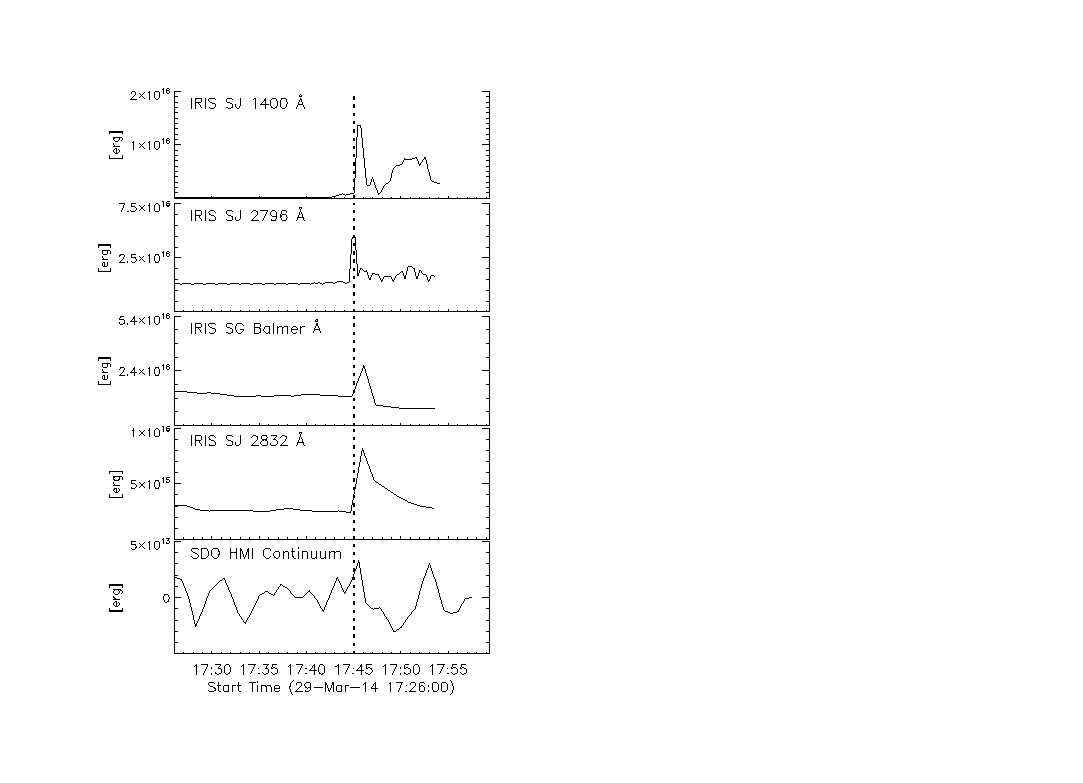
\includegraphics[width=0.8\textwidth]{29-Mar-14-Quake-Energy-Ladder}
  \end{center}
  \caption{Shows calculated energy values over time of the region thought to be the sunquake epicenter (518.5", 264.0"). Each plot represents an independant data set, in order from top to bottom the sets are; IRIS SJ 1400 \AA\ (Si IV); IRIS SJ 2796 \AA\ (Mg II); IRIS SG  2825.7 to 2825.8 \AA\ (Balmer Continuum);IRIS SJ 2832 \AA\ (Mg II wing); SDO HMI continuum (HMI).}\label{eqk}
\end{figure}
